\documentclass[10pt,conference]{ieeeconf}

%\usepackage{algpseudocode}% http://ctan.org/pkg/algorithmicx
\usepackage{xcolor}
\usepackage{subfigure}
\usepackage{amsmath,amssymb,amsbsy}
\usepackage{pdfpages}
\usepackage{epstopdf}
\usepackage{color}
\usepackage{fixmath}
\usepackage{optidef}
\usepackage{cite}
\usepackage{array,tabularx}
\usepackage{booktabs}
\usepackage[hidelinks]{hyperref}
\usepackage{cleveref}

\usepackage{color}

\ifpdf
  \RequirePackage{graphicx}
  \RequirePackage{epstopdf}
  \DeclareGraphicsExtensions{.pdf,.jpeg,.png,.jpg}
\else
  \RequirePackage[dvipdfmx]{graphicx}
  \RequirePackage{bmpsize}
  \DeclareGraphicsExtensions{.eps,.pdf,.jpeg,.png,.jpg}
\fi
\graphicspath{{pics/},{./Images/}}

\RequirePackage{algorithm}
\RequirePackage{algorithmic}
\renewcommand{\algorithmicrequire}{\textbf{Input:}}
\renewcommand{\algorithmicensure}{\textbf{Output:}}
\providecommand{\algorithmautorefname}{Algorithm}

\RequirePackage{subfigure}
\RequirePackage{empheq}
\providecommand{\subfigureautorefname}{\figureautorefname}

\providecommand{\rm}[1]{\mathrm{#1}}
\providecommand{\od}{\mathrm{d}}

\IEEEoverridecommandlockouts
\begin{document}

\title{Multichannel Deconvolution of Skin Conductance Data: Concurrent Separation of Tonic and Phasic Component}
% should be concise and informative to broad readers and attract attention from potential readers.


\author{Yuchen Jin, Jin Lu, Md. Rafiul Amin, and Rose T. Faghih \thanks{Yuchen Jin, Jin Lu, Md. Rafiul Amin, and Rose T. Faghih are with the Department of Electrical and Computer Engineering at the University of Houston, Houston, TX 77004 USA (e-mail: \tt\small  yjin4@uh.edu, jlu28@uh.edu, mamin@central.uh.edu, rtfaghih@uh.edu).} 
}

\maketitle

\begin{abstract}

The abstract should be left blank until we finish the main part of the paper.

\end{abstract}

\section{Introduction} \label{introduction}

Analyzing the electrical activities of neurons is (an important issue in the physiological field) of great interest in biomedical signal processing. By placing the electrodes, intramuscular needles or some other wearable devices, the neuron activities could be detected by different kinds of indirect methods including the electroencephalogram, electrodermal activities~\cite{savazzi2019estimation,jain2016compressed,amin2019robust}, electromyography signals~\cite{biagetti2016homomorphic}, calcium imaging, and some other approaches. The study of the neural activities could be utilized in many applications, like predicting people's emotions, monitoring the health-related abnormal events, and developing the brain-computer interface.

In this work, we concentrate on the study of electrodermal activities (EDA). EDA could be collected by measuring the skin conductance (SC) reacted to activities of people's sweat glands. The sensors for detecting EDA could be placed on either the hand palms, fingers, legs or feet. Previous works~\cite{fowles1981publication,amin2019robust} show that the EDA of different body parts is controlled by the universal neural signal from the autonomic nervous system (ANS). Within this hypothesis, the EDA could be modeled as a group of multichannel SC signals, where one chanhttps://www.overleaf.com/project/5e2b7de971963300014f339fnel represents the collected SC from a specific body part. For any channel $n$, the signal could be formulated by
\begin{align} \label{fml:scmodel}
  y_{\rm{SC}_\mathit{n}}(t) = p_n(t) + s_n(t) + \nu_n(t),
\end{align}
%
where $s_n(t)$ is the tonic component representing the influence of the body thermoregulation and also the general arousal of the body, $p_n(t)$ is the phasic component thought as reflected from the activity of ANS, and $v_n(t)$ is the additive noise. Different from the slowly drifting tonic component, the phasic component is fast-varying, which makes it possible to separate the two signals by building two different mathematical models. Both the tonic component and the phasic component could be regarded as a linear composition of different basis, or a group of kernels convoluted on spike signals in time series. It is possible to formulate a deconvolution problem with the physiological interpretation of SC, which requires a solution for the ANS activation given the composed signal  $y_{\rm{SC}_n}(t)$  is known.

\subsection{Deconvolution}

The neural stimuli from the ANS is though as spike signals. While after the signal is conducted to the sweat glands, the signals are smoothly filtered due to the (physiological effects) physiological systems. After applying the deconvolution, the estimated neural stimuli could be used for denoising, emotion predictions, or health monitoring. \textit{Caruelle et al.}~\cite{caruelle2019use} summarizes the applications of the EDA analysis in recent years. For more details, \textit{Posada et al.}~\cite{posada2020innovations} provides a review on the previous deconvolution methods with the EDA data. Similar to EDA, the other kinds of signals could be also used for studying the neuron activities by deconvolution. In \cref{tab:literature}, we inspect on several works on deconvolution with different data. For the simplest case, the spike signal could be retrieved by applying a threshold and performing the local maximum searching~\cite{kaur2016remote,subramanian2019systematic}. In most works, the deconvolution is solved by formulating an optimization problem based on a linear model, including the Bateman function~\cite{savazzi2019estimation,greco2014electrodermal,greco2015cvxeda,amin2019tonic,hernando2017feature,wickramasuriya2019skin}, the AR-1 model~\cite{friedrich2017fast}, and the state-space model~\cite{kazemipour2017fast,amin2019robust}. 

The complexity of the deconvolution differs in different applications. In \cite{greco2015cvxeda}, the basis determining the shape of the phasic component is fixed., while in \cite{hernando2017feature}, the phasic component is modeled by several fixed bases. In \cite{greco2014electrodermal,amin2019tonic,wickramasuriya2019skin,kazemipour2017fast,amin2019robust}, although there is a single basis, the shape of the basis could be learned. Particularly, some researches assume that the linear model is totally unknown. By only giving an initial guess, the modeling function is also optimized by blind deconvolution~\cite{kaur2016remote,friedrich2017fast}. For a large scale application, the problem requires to be formulated properly according to the computational consumption.

Most of the mentioned works are dealing with single channel data, while in \cite{friedrich2017fast,amin2019robust}, a multichannel scheme is introduced for improving the robustness of the predictions. In the practice, observations are mixed with the noise, which may influence the accuracy of the deconvolved spikes. The motivation of introducing multichannel data is based on the hypothesis that the same neural stimuli is shared by the data acquired by different observations. When the multichannel data is deconvolved jointly, the noise from different channels could be attenuated by each other, thus the problem could converge on a better solution.

\begin{table*}[htbp]
  \centering
  \normalsize
  \caption{A summary of the previous works about deconvolution.}
  \label{tab:literature}
  \begin{tabular}{m{0.14\textwidth}<{\raggedright}m{0.14\textwidth}<{\raggedright}m{0.65\textwidth}}
    \toprule
    \multicolumn{1}{c}{Study} & \multicolumn{1}{c}{Data} & \multicolumn{1}{c}{Methodology} \\ \midrule
    \textit{Friedrich et. al.}~\cite{friedrich2017fast} & Calcium imaging data & The conversion from the calcium spikes to the observed fluorescenc signals is described as an AR-p model. The authors propose an algorithm, OASIS for solving the constrained optimization problem in the AR-1 case. \\
    \textit{Kazemipour et. al.}~\cite{kazemipour2017fast} & Calcium imaging data & Develop a compressible state-space model for describing the data. The spikes are designed as the innovation sequence of the state. The optimization problem is solved by a nested Expectation-Maximization algorithm. \\
    \textit{Kaur et. al.}~\cite{kaur2016remote} & Electro-cardiogram & Introduce two methods. The first method is based on curve fitting and local maximum searching. The second method is Blind Deconvolution, where the kernel and the spikes are optimized alternatively. \\
    \textit{Mesin}~\cite{mesin2019single} & Electromyogram & Model the EMG signal by motor unit kernels. The deconvolution is performed by solving an $\ell_1$ regularized optimization problem by the iterative reweighted least square algorithm. \\
    \textit{Antink et. al.}~\cite{friedrich2017fast} & ECG, ABP and PPG & The author use the blind deconvolution to solve the heart beat spikes. This paper introduces a multi-observation scheme by assuming a universal spike data. \\
    \textit{Subramanian et. al.}~\cite{subramanian2019systematic} & EDA & Use a low-pass FIR filter to isolate the tonic component, the spike is found by searching local maximum in phasic component. \\ 
    \textit{Savazzi et. al.}~\cite{savazzi2019estimation} & EDA & The tonic component and noise is removed by a low-pass FIR filter. The phasic component is modeled by Bateman function. The spike is acquired by optimization. \\ 
    \textit{Jain et. al.}~\cite{jain2016compressed} & EDA & Involve the compress sensing into the deconvolution. The optimization is performed on the differential signal to eliminate the influence of sudden changes of the tonic component. \\
    \textit{Greco et. al.}~\cite{greco2014electrodermal} & EDA & The tonic component is estimated by Gaussian smoothing and interpolation. The spike is solved by modeling the phasic component with Bateman function. \\ 
    \textit{Greco et. al.}~\cite{greco2015cvxeda}, \textit{Amin and Faghih}~\cite{amin2019tonic} & EDA & Model the phasic component and the tonic component by Bateman function and spline function respectively, then formulate the deconvolution as a joint constrained convex optimization problem. \\ 
    \textit{Hernando et. al.}~\cite{hernando2017feature} & EDA & The tonic and phasic components are decomposed by two groups of pre-defined bases. The phasic component basis is designed by using Bateman function. \\
    \textit{Wickramasuriya et. al.}~\cite{wickramasuriya2019skin} & EDA & The tonic component is isolated by using cvxEDA~\cite{greco2015cvxeda}. The phasic component is decomposed by a basis based on Bateman function. The deconvolution is solved by a hybrid algorithm based on GCV and FOCUSS+. \\
    \textit{Amin and Faghih}~\cite{amin2019robust} & EDA & The authors propose a multichannel deconvotion scheme. The tonic component is removed by using cvxEDA~\cite{greco2015cvxeda} on each channel, and the phasic component is formulated by a state-space model. The deconvolution is solved by the hybrid algorithm GCV-FOCUSS+. \\ \bottomrule
  \end{tabular}
\end{table*}

\subsection{Tonic separation}
 
Previously there some works on the tonic component separation. In \cite{van1967skin}, the raw EDA signal is decomposed as absolute change in conductance, change as a ratio of the basic conductance level (BLC), and log conductance change. In \cite{green2014development}, the author proposes a method of automated analysis of SCR data in the contexts of event-related cognitive tasks and nonspecific responding to complex stimuli. \cite{greco2014electrodermal} formulates the separation as a quadratic programming problem, where the phasic component and the tonic component are decomposed by the basis of the biexponential Bateman functions and the B-spline functions respectively. To solve the problem that the tonic component may overlap each other, \textit{Vartak et. al.}~\cite{vartak2009estimation} proposes a mathematical model fitting procedure is used to separate these overlapping components. Features are extracted using the mathematical model fitting procedure. In~\cite{amin2019tonic}, the author proposes a generalized-cross-validation-based block coordinate descent approach. In this approach, the tonic component is regarded as a summation of a series of P shifted and weighted cubic B-spline functions. Then the problem is solved by minimizing an $\ell_p$ penalized loss function. Especially, inspired by compress sensing, \textit{Jain et. al.}~\cite{jain2016compressed} builds a model for separating the difference of the signal instead of the raw signal. This idea is effective for eliminating the interference caused by sudden changes of the tonic component.

In some previous works, the tonic component separation and the phasic component deconvolution are performed individually~\cite{greco2014electrodermal,amin2019robust}. Since both the modeling method and the inversion method in \cite{amin2019robust} are designed for the multichannel case, the previous tonic separation works designed for single-channel data may cause deviation for the solution. In addition to the motivation, we are interested in multi-channel deconvolution inorder to obtain more accurate results in presence of noise. As tonic component separation is performed separately, inaccuracy in separation in presence of artifact and noise may lead to inaccurate deconvolution of ANS activation. A multi-channel tonic and phasic decomposition may lead to a more robust decomposition in presence of noise. In our work, we extend the multichannel deconvolution into the joint optimization for solving the tonic component in the multichannel case. With this scheme, the neural stimuli from the ANS is though to be shared, while the solution for the composition of tonic basis is assumed to be different in different channels.

\section{Theory}

According to \eqref{fml:scmodel}, the SC data could be decomposed into a tonic component and a phasic component. In this work, we will model both components by different methods. The phasic component is decomposed by a series of state-space models sharing the same input, while the tonic component is described as a combination of different spline functions. Based on the theory-based multichannel forward modeling, the stimuli from the ANS could be solved by a joint optimization. In the meanwhile, the tonic component would be extracted from the data.

\subsection{Model the phasic component with a multichannel state-space representation}
According to the presumption in \cite{alexander2005separating,society2012publication,amin2019robust}, the phasic components detected in different regions of the body are regulated by the same ANS signal, the detected phasic component for channel $n$ could be formulated by
\begin{align}
p_n(t) = \alpha_n \zeta_n (t),
\end{align}
where $\alpha_n$ denotes the attenuation caused by the the different number and sizes of sweat glands in different location. $\zeta_n(t)$ is an internal variable which is modeled by a smoothing filter applied to the neural stimuli $u(t-\beta_n)$. The conduction delay $\beta_n$ shows that the same stimuli would be detected at different moments. Generally, the neural stimuli could be defined as a time-series spike signal, i.e. $u(t) = \sum_{i=1}^N q_i \delta(t - \Delta_i)$, where $q_i$ is the spike signal in time interval i, and $\Delta_i$ is the time for ith time interval. Given $u(t)$, \textit{Alexander et al.}~\cite{alexander2005separating} provides a second-order ordinary differential equation to describe $\zeta_n(t)$,
\begin{align} \label{fml:the:ode}
\tau_r \tau_d \frac{\od^2 \zeta_n(t)}{\od t^2} + (\tau_r + \tau_d) \frac{\od \zeta_n(t)}{\od t} + \zeta_n(t) = u(t - \beta_n).
\end{align}

The difference between different channels in \eqref{fml:the:ode} is only the time delay. In other words, the solutions of $\zeta_n(t)$ for different $n$ are the same except the time delay. To solve \eqref{fml:the:ode}, \textit{Faghih et al.}~\cite{faghih2015characterization} propose a state space model. Incorporating the time delay into the internal signal $\zeta_n(t)$, we denote another internal state $x^{(n)}_2 (t)$ as $\zeta_n(t + \beta_n)$. The state-space model could be formulated as the following form,
\begin{subequations} \label{fml:the:state-raw}
  \renewcommand{\theequation}
  {\theparentequation-\arabic{equation}}
  \begin{empheq}[left=\empheqlbrace]{align}
  \dot{x}^{(n)}_1 (t) &= a x^{(n)}_1(t) + b u(t),\\
  \tau_r \tau_d \dot{x}^{(n)}_2 (t) &= c x^{(n)}_1(t) + d x^{(n)}_2(t), \label{fml:the:state-raw-2}\\
  y_n (t) &= \alpha_n x^{(n)}_2(t).
  \end{empheq}
\end{subequations}
{\color{red} I have to say that I do not know why we design \eqref{fml:the:state-raw}.}

where $x^{(n)}_1(t)$ is another internal state. To solve the coefficients $a, b, c, d$, we eliminate $x^{(n)}_1(t)$ in \eqref{fml:the:state-raw-2},
\begin{equation} \label{fml:the:ode-from-state}
\begin{aligned}
\tau_r \tau_d \ddot{x}_2 (t) &= c \dot{x}^{(n)}_1(t) + d \dot{x}^{(n)}_2(t) \\
&= c \left(a x^{(n)}_1(t) + b u(t) \right) + d \dot{x}^{(n)}_2(t) \\
&= a ( \tau_r \tau_d \dot{x}^{(n)}_2 (t) - d x^{(n)}_2(t) ) + bc u(t) + d \dot{x}^{(n)}_2(t), \\
&= (a \tau_r \tau_d + d) \dot{x}^{(n)}_2 (t) - a d x^{(n)}_2(t) + bc u(t).
\end{aligned}
\end{equation}

To ensure the coherence between \eqref{fml:the:ode} and \eqref{fml:the:ode-from-state}, we have,
\begin{subequations}
  \renewcommand{\theequation}
  {\theparentequation-\arabic{equation}}
  \begin{empheq}[left=\empheqlbrace]{align}
  a \tau_r \tau_d + d &= - \tau_r - \tau_d,\\
  ad &= 1, \\
  bc &= 1. 
  \end{empheq}
\end{subequations}

Given $a = -1/\tau_r$ and $b = 1/\tau_r$, we could solve the above equations, and substitute the solutions into \eqref{fml:the:state-raw},
\begin{subequations} \label{fml:the:state-sing}
  \renewcommand{\theequation}
  {\theparentequation-\arabic{equation}}
  \begin{empheq}[left=\empheqlbrace]{align}
    &\begin{aligned}
      \begin{bmatrix}
        \dot{x}^{(n)}_1 (t) \\ \dot{x}^{(n)}_2 (t)
      \end{bmatrix} &= \begin{bmatrix}
        -1/{\tau_r} & 0 \\ 1/{\tau_d} & -1/{\tau_d}
      \end{bmatrix} \begin{bmatrix}
        x^{(n)}_1(t) \\ x^{(n)}_2 (t)
      \end{bmatrix} \\ &+ \begin{bmatrix}
        1/{\tau_r} \\ 0
      \end{bmatrix} u(t), 
    \end{aligned} \\
    &y_n (t) = \alpha_n x^{(n)}_2(t).
  \end{empheq}
\end{subequations}

Given the single-channel transmission matrix $\phi=\begin{bmatrix}
-1/{\tau_r} & 0 \\ 1/{\tau_d} & -1/{\tau_d}
\end{bmatrix}$, we could derive \eqref{fml:the:state-sing} into the multichannel form. When we have $\chi$ channels of data, the multichannel state-space model is
\begin{subequations} \label{fml:the:state-mul}
  \renewcommand{\theequation}
  {\theparentequation-\arabic{equation}}
  \begin{empheq}[left=\empheqlbrace]{align}
  \dot{\mathbf{x}} (t) &= \mathbf{A} \mathbf{x} (t) + \mathbf{B} u (t), \\
  \mathbf{y} (t) &= \mathbf{C} \mathbf{x} (t),
  \end{empheq}
\end{subequations}
where $\mathbf{x} (t) = \begin{bmatrix}
x^{(1)}_1 (t) \\ x^{(1)}_2 (t) \\ \vdots \\ x^{(\chi)}_1 (t) \\ x^{(\chi)}_2 (t)
\end{bmatrix}$, $\mathbf{y} (t) = \begin{bmatrix}
y_1 (t) \\ y_2 (t) \\ \vdots \\ y_{\chi} (t)
\end{bmatrix}$, $\mathbf{A} = \begin{bmatrix}
\phi & \mathbf{0} & \cdots & \mathbf{0} \\
\mathbf{0} & \phi & \cdots & \mathbf{0} \\
\vdots & \vdots & \ddots & \vdots \\
\mathbf{0} & \mathbf{0} & \cdots & \phi
\end{bmatrix}$, $\mathbf{B} = \begin{bmatrix}
1/{\tau_r} \\ 0 \\ \vdots \\ 1/{\tau_r} \\ 0
\end{bmatrix}$, and\\$\mathbf{C} = \begin{bmatrix}
0 & \alpha_1 & 0 & 0 & \cdots & 0 & 0 \\ 0 & 0 & 0 & \alpha_2 & \cdots & 0 & 0 \\ \vdots & \vdots & \vdots & \vdots & \ddots & \vdots & \vdots \\ 0 & 0 & 0 & 0 & \cdots & 0 & \alpha_{\chi}
\end{bmatrix}$.

The above model could be rewritten as a discrete model. Denote the sampling rates of the observation and the neural stimuli as $T_y$ and $T_u$ respectively, we could formulate the discretion of the time as $t_k = k T_y$ and $\Delta_i = i T_u$ for both signals. When $T_u$ is small enough, we could approximate the discrete neural stimuli by $\mathbf{u} = \begin{bmatrix}
u_1 & u_2 & \cdots & u_N
\end{bmatrix}^T$, where we use $u_i=0$ to represent no signal at the time step $\Delta_i$. Based on these configurations, we could derive the discrete model matrices by
\begin{subequations} \label{fml:the:state-dis-mat}
  \renewcommand{\theequation}
  {\theparentequation-\arabic{equation}}
  \begin{empheq}[left=\empheqlbrace]{align}
  \mathcal{A} &= \mathcal{L}^{-1}\{ \left(s \mathbf{I} - \mathbf{A} \right)^{-1} \}(T_u), \\
  \mathcal{B} &= \mathbf{A}^{-1}(\mathcal{A} - \mathbf{I})\mathbf{B}, \\
  \mathcal{C} &= \mathbf{C},
  \end{empheq}
\end{subequations}
where $\mathcal{L}^{-1}$ is the inverse Laplace transform.
{\color{red} I have checked~\cite{wikidiscreteize} and fix the equation \eqref{fml:the:state-dis-mat}.}

The discrete form of \eqref{fml:the:state-mul} is
\begin{subequations} 
  \renewcommand{\theequation}
  {\theparentequation-\arabic{equation}}
  \begin{empheq}[left=\empheqlbrace]{align}
  \mathbf{x} [k+1] &= \mathcal{A} \mathbf{x} [k] + \mathcal{B} \mathbf{u} [k], \\
  \mathbf{y} [k] &= \mathcal{C} \mathbf{x} [k],
  \end{empheq}
\end{subequations}

In practice, we assume that $T_y = L T_u$, where $L$ is an integer. In this case, we could denote the state vector based on the sampling rate $T_y$ by $\mathbf{z}[k] = \mathbf{x}[Lk]$. Then we have $\mathcal{A}_d = \mathcal{A}^L$, $\mathcal{B}_d = \begin{bmatrix}
\mathcal{A}^{L-1} \mathcal{B} & \mathcal{A}^{L-2} \mathcal{B} & \cdots \mathcal{B}
\end{bmatrix}$, $\mathbf{u}_d[k] = \begin{bmatrix}
\mathbf{u}[Lk] & \mathbf{u}[Lk+1] & \cdots \mathbf{u}[Lk+L-1]
\end{bmatrix}^T$. By this way, the discrete model is finally formulated as
\begin{subequations} \label{fml:the:state-dis}
  \renewcommand{\theequation}
  {\theparentequation-\arabic{equation}}
  \begin{empheq}[left=\empheqlbrace]{align}
  \mathbf{z} [k+1] &= \mathcal{A}_d \mathbf{z} [k] + \mathcal{B}_d \mathbf{u}_d [k], \\
  \mathbf{y} [k] &= \mathcal{C} \mathbf{z} [k],
  \end{empheq}
\end{subequations}

Since the system is casual, we have
\begin{align} \label{fml:the:out-dis}
\mathbf{y}[k] = \mathcal{F}[k] \mathbf{z}_0 + \mathcal{D}[k] \mathbf{u},
\end{align}
where $\mathcal{F}[k] = \mathcal{C}\mathcal{A}_d^k$, $\mathcal{D}[k] = \mathcal{C} \begin{bmatrix}
\mathcal{A}_d^{k-1} \mathcal{B}_d & \mathcal{A}_d^{k-2} \mathcal{B}_d & \cdots \mathcal{B}_d & \mathbf{0}_{N-kL}
\end{bmatrix}$ and \\$\mathbf{u} = \begin{bmatrix}
\mathbf{u}_d[0] & \mathbf{u}_d[1] & \cdots & \mathbf{u}_d[M-1]
\end{bmatrix}^T$. The initial condition is configured as \\$\mathbf{z}_{0} = \mathbf{z}[0] = \begin{bmatrix}
0 & y_1(0) & 0 & \frac{y_2(0)}{\alpha_2} & \cdots & 0 & \frac{y_{\chi}(0)}{\alpha_{\chi}}
\end{bmatrix}^T$.

Let $\mathbf{y} = \begin{bmatrix}
\mathbf{y}[1]^T & \mathbf{y}[2]^T & \cdots & \mathbf{y}[M]^T
\end{bmatrix}^T$, $\mathcal{F}_{\boldsymbol{\theta}} = \begin{bmatrix}
\mathcal{F}[0] & \mathcal{F}[1] & \cdots & \mathcal{F}[M-1]
\end{bmatrix}^T$ and \\$\mathcal{D}_{\boldsymbol{\theta}} = \begin{bmatrix}
\mathcal{D}[0] & \mathcal{D}[1] & \cdots & \mathcal{D}[M-1]
\end{bmatrix}^T$, we can represent the whole multichannel phasic component by
\begin{align} \label{fml:the:out-dis-all}
\mathbf{y} = \mathcal{F}_{\boldsymbol{\theta}} \mathbf{z}_{0} + \mathcal{D}_{\boldsymbol{\theta}} \mathbf{u},
\end{align}
where we use $\boldsymbol{\theta}$ to denote the learnable vector $\begin{bmatrix}
\tau_r & \tau_d & \alpha_1 & \alpha_2 & \cdots & \alpha_{\chi}
\end{bmatrix}^T$.

\subsection{Model the tonic component with spline functions}

The tonic signal of the $n^{\mathrm{th}}$ channel could be viewed as the coefficients $q_n (t)$ convolved with the cubic B-spline function $\psi(t)$,
\begin{align}
s_n(t) =  \psi(t) \otimes q_n (t).
\end{align}

The coefficients could be viewed as a time-series signal composed of several spikes, i.e. $q_n (t) = \sum_{j=1}^K q_{nj} \delta(t - jT_s)$, where $T_s$ is the sampling rate of the coefficients. $T_s$ could be used to control the smoothness of the B-spline function. To ensure the smoothness, we usually use a longer period for $T_s$ like 5s. With these configurations, we could discretize the coefficients as $\tilde{\mathbf{q}}_n = \begin{bmatrix}
q_{n1} & q_{n2} & \cdots q_{nK}
\end{bmatrix}^T$.
The convolution on $\psi(t)$ could be formulated by a Toeplitz matrix $\tilde{\mathbf{C}}$. The $m^{\mathrm{th}}$ row of the matrix could be formulated as
\begin{align}
\tilde{\mathbf{c}}_m = \begin{bmatrix}
\psi(mT_y + T_s) & \psi(mT_y) & \cdots & \psi(T_u - T_s)
\end{bmatrix}.
\end{align}

We follows the work in~\cite{greco2015cvxeda}, where two linear trend parameters are introduced for solving the tonic component. Given the following linear trend matrix,
\begin{align}
  \mathbf{R} = \begin{bmatrix}
    1/K & 2/K & 3/K & 4/K & \cdots & 1 \\
    1 & 1 & 1 & 1 & \cdots & 1 
  \end{bmatrix}.
\end{align}

Then we could formulate the tonic component as
\begin{align}
\mathbf{s}_n = \mathbf{C} \mathbf{q}_n = \begin{bmatrix}
  \tilde{\mathbf{C}} & \mathbf{R}
\end{bmatrix} \begin{bmatrix}
  \tilde{\mathbf{q}}_n \\ r_{1n} \\ r_{0n}
\end{bmatrix}.
\end{align}

\subsection{Preprocess the data}

Preprocessing aims at removing the outliers in the raw data. The whole process is shown in \cref{alg:preprocessing}. We find the peaks of the differentiated raw data. The searching method is based on comparing the 2 values near the center point. The data patches with outliers are all replaced by their spline approximations. Most of the outliers could be removed by this way.
\begin{algorithm}[tb]
  \caption{The preprocessing applied to the raw data.}
  \label{alg:preprocessing}
  \begin{algorithmic}[1]
    \REQUIRE The raw data $\{\mathbf{y}_{\mathrm{SC}_n}\}_{n=1}^\chi$ for $\chi$ channels.
    \ENSURE The preprocessed data $\{\hat{\mathbf{y}}_{\mathrm{SC}_n}\}_{n=1}^\chi$ for $\chi$ channels.
    % if-then-else
    \FOR{$n$ from $1$ to $\chi$}
    \STATE Find the local positive and negative peaks of the differential data $\dot{\mathbf{y}}_{\mathrm{SC}_n}$, where peaks means the data with a value larger than the around values by 0.1;
    \FORALL{founded peaks}
    \STATE Select 4 points near the peak, the range is limited in 100 points around the peak;
    \STATE Use the spline interpolation of the selected 4 points to replace the 100 points;
    \ENDFOR
    \STATE Perform the 64 order low-pass FIR filter, the cut-off frequency is 3 Hz;
    \ENDFOR
  \end{algorithmic}
\end{algorithm}

\subsection{Solve the deconvolution}

After modeling the data by the aforementioned two methods, we could formulate the $n^{\mathrm{th}}$ channel of the SC data as follows,
\begin{align}
\mathbf{y}_n = \mathcal{F}_{\boldsymbol{\theta}_n} \mathbf{z}_{0} + \mathcal{D}_{\boldsymbol{\theta}_n} \mathbf{u} + \mathbf{C} \mathbf{q}_n + \boldsymbol{\nu}_n,
\end{align}
where $\boldsymbol{\theta}_n = \begin{bmatrix}
\tau_r & \tau_d & \alpha_n
\end{bmatrix}^T$ is the subset of the learnable vector $\boldsymbol{\theta}$, $\mathbf{q}_n$ is the decomposition coefficients of the $n^{\mathrm{th}}$ tonic component and $\boldsymbol{\nu}_n$ is the noise vector for $n^{th}$ channel. Typically $\boldsymbol{\nu}_n$ could be approximated by the Gaussian random noise. For the phasic decomposition, the coefficients, i.e. the neural stimuli $\mathbf{u}$ is shared, and the model parameters are not totally shared crossing the channels. For the tonic decomposition, the modeling function $\mathbf{C}$ is shared crossing the channels, while the coefficients $\mathbf{q}_n$ are different among different channels.

The multichannel deconvolution with the tonic separation could be formulated by the following constrained joint optimization problem,
\begin{subequations} \label{fml:the:optimization}
  \renewcommand{\theequation}
  {\theparentequation-\arabic{equation}}
  \begin{align}
  \arg\min\limits_{\substack{\boldsymbol{\theta},~\mathbf{u}, \\ \{\mathbf{q}_n\}_{n=1}^{\chi}, \\ \lambda,~\{\mu_n\}_{n=1}^{\chi}}} & \frac{1}{\chi} \left( \sum_{n=1}^{\chi} \mathcal{J}_n + \mu_n \lVert \mathbf{q}_n \rVert_2^2 \right) + \lambda \lVert \mathbf{u} \rVert^p_p, \\
  \mathrm{s.t.}~&\mathcal{J}_n = \lVert \mathbf{y}_n - \mathcal{F}_{\boldsymbol{\theta}_n} \mathbf{z}_{0} - \mathcal{D}_{\boldsymbol{\theta}_n} \mathbf{u} - \mathbf{C} \mathbf{q}_n \rVert^2_2, \label{fml:loss-channel}\\
  & \boldsymbol{\Gamma} \boldsymbol{\theta} \preccurlyeq \mathbf{b},~ \mathbf{u} \succcurlyeq \mathbf{0} \label{fml:cons-phasic}\\
  & \forall~n,~\mathbf{q}_n \succcurlyeq \mathbf{0},~\mathbf{C}\mathbf{q}_n \preccurlyeq \mathbf{y}_n, \label{fml:cons-tonic}
  \end{align}
\end{subequations}
where \eqref{fml:loss-channel} represents the loss function for the $n^{\mathrm{th}}$ channel, \eqref{fml:cons-phasic} is the constraint of the phasic decomposition, and \eqref{fml:cons-tonic} is the constraint of the tonic extraction. In \eqref{fml:cons-phasic}, the Tikhonov matrix $\boldsymbol{\Gamma}$ and the boundary vector $\mathbf{b}$ are defined as
\begin{subequations} \label{fml:the:constraint}
  \renewcommand{\theequation}
  {\theparentequation-\arabic{equation}}
  \begin{align}
  \boldsymbol{\Gamma} &= \begin{bmatrix}
  1 & -1 & 0 & 0 & \cdots & 0 & 0 \\
  0 & 0 & 1 & -1 & \cdots & 0 & 0 \\
  \vdots & \vdots & \vdots & \vdots & \ddots & \vdots & \vdots \\
  0 & 0 & 0 & 0 & \cdots & 1 & -1
  \end{bmatrix}, \\
  \mathbf{b} &= 
    \begin{array}{ccccc}
      \big[1.4 & -0.1 & 6.0 & -1.5 & 100.0 \\
      & -0.01 & \cdots & 100.0 & -0.01 \big]^T
    \end{array}  
  \end{align}
\end{subequations}

Conventionally, it is difficult to decide the proper the regularization coefficients $\lambda,~\mu_n$. In our work, we take the optimization of the coefficients into the consideration. The optimization is based on Focal Underdetermined System Solver (FOCUSS+) algorithm~\cite{murray2005visual}, while the estimation of the tunable regularization coefficients is based on  generalized cross-validation (GCV) method~\cite{zdunek2008improved}. 

The whole algorithm for the optimization is discussed in \cref{alg:deconvolution}. The algorithm has 2 phases. In the first phase, we use a simpler method to find a good initialization. In this case, the tonic component and the phasic component are solved separately. The approximated solution for tonic component could be formulated by
\begin{subequations} \label{fml:the:firststage}
  \renewcommand{\theequation}
  {\theparentequation-\arabic{equation}}
  \begin{align}
  \arg \min\limits_{\mathbf{q}_n,~\mu_n} & \lVert \mathbf{y}_n - \mathbf{C} \mathbf{q}_n \rVert^2_2 + \mu_n \lVert \mathbf{q}_n \rVert_2^2, \\
  \mathrm{s.t.}~& \forall~n,~\mathbf{q}_n \succcurlyeq \mathbf{0},~\mathbf{C}\mathbf{q}_n \preccurlyeq \mathbf{y}_n.
  \end{align}
\end{subequations}

In the second phase, the optimization could be divided into an outer loop and an inner loop. In the outer loop, we solve the modeling parameters $\boldsymbol{\theta}$. The deconvolution and with the tonic extraction is performed in the inner loop. Particularly, given the solution of $\mathbf{q}_n$, when solving the tonic component, for any $n$, we need to solve the following constrained quadratic problem,
\begin{subequations} \label{fml:the:second-tonic}
  \renewcommand{\theequation}
  {\theparentequation-\arabic{equation}}
  \begin{align}
  \arg \min\limits_{\mathbf{q}_n,~\mu_n} & \lVert \mathbf{s}_n - \mathbf{C} \mathbf{q}_n \rVert^2_2 + \mu_n \lVert \mathbf{q}_n \rVert_2^2, \\
  \mathrm{s.t.}~& \mathbf{s}_n = \max\left( \mathbf{y}_n - \mathcal{F}_{\boldsymbol{\theta}_n} \mathbf{z}_{0} - \mathcal{D}_{\boldsymbol{\theta}_n} \mathbf{u},~\mathbf{C} \mathbf{q}^{(0)}_n \right), \label{fml:the:second-tonic-obj}\\
  & \forall~n,~\mathbf{q}_n \succcurlyeq \mathbf{0},~\mathbf{C}\mathbf{q}_n \preccurlyeq \mathbf{y}_n,
  \end{align}
\end{subequations}
%
where $\mathbf{q}^{(0)}_n$ is the initial guess solved by the first phase. We use this technique to guarantee that the solution of the tonic component $\mathbf{C} \mathbf{q}_n$ lower bounded by the initial solution.

When solving the phasic component, we make the tonic component fixed, and solve the following problem,
\begin{subequations} \label{fml:the:second-phasic}
  \renewcommand{\theequation}
  {\theparentequation-\arabic{equation}}
  \begin{align}
  \arg \min\limits_{\boldsymbol{\theta},~\mathbf{u},~\lambda} & \frac{1}{\chi}  \left( \sum_{n=1}^{\chi} \lVert \mathbf{p}_n - \mathcal{F}_{\boldsymbol{\theta}_n} \mathbf{z}_{0} - \mathcal{D}_{\boldsymbol{\theta}_n} \rVert^2_2 \right) + \lambda \lVert \mathbf{u} \rVert_p^p, \\
  \mathrm{s.t.}~& \mathbf{p}_n = \mathbf{y}_n -  \mathbf{C} \mathbf{q}_n, \\
  & \boldsymbol{\Gamma} \boldsymbol{\theta} \preccurlyeq \mathbf{b},~ \mathbf{u} \succcurlyeq \mathbf{0}.
  \end{align}
\end{subequations}

To solve the joint problem in \eqref{fml:the:optimization}, we need to solve \eqref{fml:the:second-tonic} and \eqref{fml:the:second-phasic} alternatively. This technique is called concurrent coordinate descent method.

\begin{algorithm}[!tb]
  \caption{The preprocessing applied to the raw data.}
  \label{alg:deconvolution}
  \begin{algorithmic}[1]
    \REQUIRE The preprocessed multichannel data $\{\hat{\mathbf{y}}_{\mathrm{SC}_n}\}_{n=1}^\chi$, the decomposition coefficients $\mathbf{u}, \{\mathbf{q}_{n}\}_{n=1}^\chi$, and the initialized parameters $\boldsymbol{\theta}$, where $\tau_d \sim U(0.10,~1.4)$, $\tau_r \sim U(1.5,~6.0)$, $\alpha_n \sim U(0.01,~1.0)$, $\mathbf{u} \sim 0$, and $\mathbf{q}_n \sim \mathcal{N}(0.1, 0.02)$.
    % if-then-else
    \STATE Ignore $\boldsymbol{\theta},~\mathbf{u}$ and let $\mu_n$ fixed. For any $n$, use interior point method to solve $\{\mathbf{q}_{n}\}$ from \eqref{fml:the:firststage};
    \FOR {$j$ from $1$ to $30$}
      \STATE Let $\boldsymbol{\theta},~\{\mathbf{q}_{n}\}$ fixed, use FOCUSS+ to solve $\tilde{\mathbf{u}}^{(j)}$ from \eqref{fml:the:optimization}. Set $\mathbf{u} = \tilde{\mathbf{u}}^{(j)}$;
      \STATE Let $\mathbf{u},~\{\mathbf{q}_{n}\}$ fixed, solve $\tilde{\boldsymbol{\theta}}^{(j)}$ from \eqref{fml:the:optimization} by the interior point method. Set $\boldsymbol{\theta} = \tilde{\boldsymbol{\theta}}^{(j)}$;
    \ENDFOR
    \STATE Initialize $\hat{\boldsymbol{\theta}}^{(0)}=\boldsymbol{\theta}$, $\hat{\mathbf{u}}^{(0)}=\mathbf{u}$, $\{\hat{\mathbf{q}}_{n}\}^{(0)}=\{\mathbf{q}_{n}\}$;
    \FOR{$i$ from $0$ until converge}
      \STATE Let $\hat{\mu}^{(i)(0)} = 2 \times 10^{-3}$,
      \FOR{$m$ from $1$ until converge}
      \STATE Let $\mu = \hat{\mu}^{(i)(m-1)}$, $\boldsymbol{\theta},\mathbf{u}$ fixed, use interior point method to solve $\{\hat{\mathbf{q}}_{n}\}^{(i)(m)}$ from \eqref{fml:the:second-tonic}. Set $\{\mathbf{q}_{n}\} = \{\hat{\mathbf{q}}_{n}\}^{(i)(m)}$;
      \STATE Let $\mathbf{u},~\boldsymbol{\theta}~\{\mathbf{q}_{n}\}$ fixed, use GCV to solve $\hat{\mu}^{(i)(m)}$. Set $\mu = \hat{\mu}^{(i)(m)}$;
      \ENDFOR
      \STATE Set $\{\hat{\mathbf{q}}_{n}\}^{(i)} =  \{\hat{\mathbf{q}}_{n}\}^{(i)(m)}$.
      \STATE Let $\boldsymbol{\theta},~\{\mathbf{q}_{n}\}$ fixed, solve $\hat{\mathbf{u}}^{(j)}$ by the following steps;
      \STATE Let $\hat{\lambda}^{(i)(0)} = 2 \times 10^{-3}$,
      \FOR{$m$ from $1$ until converge}
      \STATE Let $\lambda = \hat{\lambda}^{(i)(m-1)}$, $\boldsymbol{\theta},~\{\mathbf{q}_{n}\}$ fixed, use FOCUSS+ to solve $\hat{\mathbf{u}}^{(i)(m)}$ from \eqref{fml:the:second-phasic}. Set $\mathbf{u} = \hat{\mathbf{u}}^{(i)(m)}$;
      \STATE Let $\mathbf{u},~\boldsymbol{\theta}~\{\mathbf{q}_{n}\}$ fixed, use GCV to solve $\hat{\lambda}^{(i)(m)}$. Set $\lambda = \hat{\lambda}^{(i)(m)}$;
      \ENDFOR
      \STATE Set $\hat{\mathbf{u}}^{(i)} = \hat{\mathbf{u}}^{(i)(m)}$.
    \ENDFOR
  \end{algorithmic}
\end{algorithm}

\section{Results}

\begin{figure*}[htbp]
  \centering
  \subfigure[Reconstructed signal for the thenar/hypothenar data.]{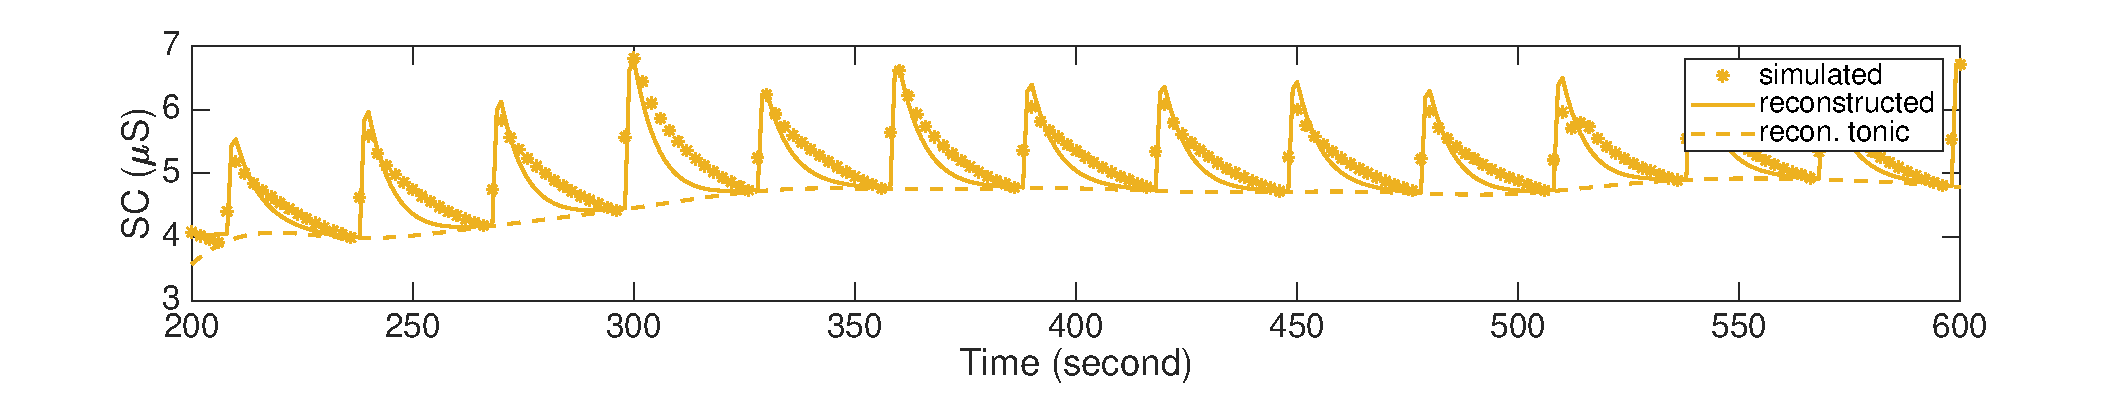
\includegraphics[width=0.9\textwidth]{thenar}}
  \subfigure[Reconstructed signal for the volar middle phalanx data.]{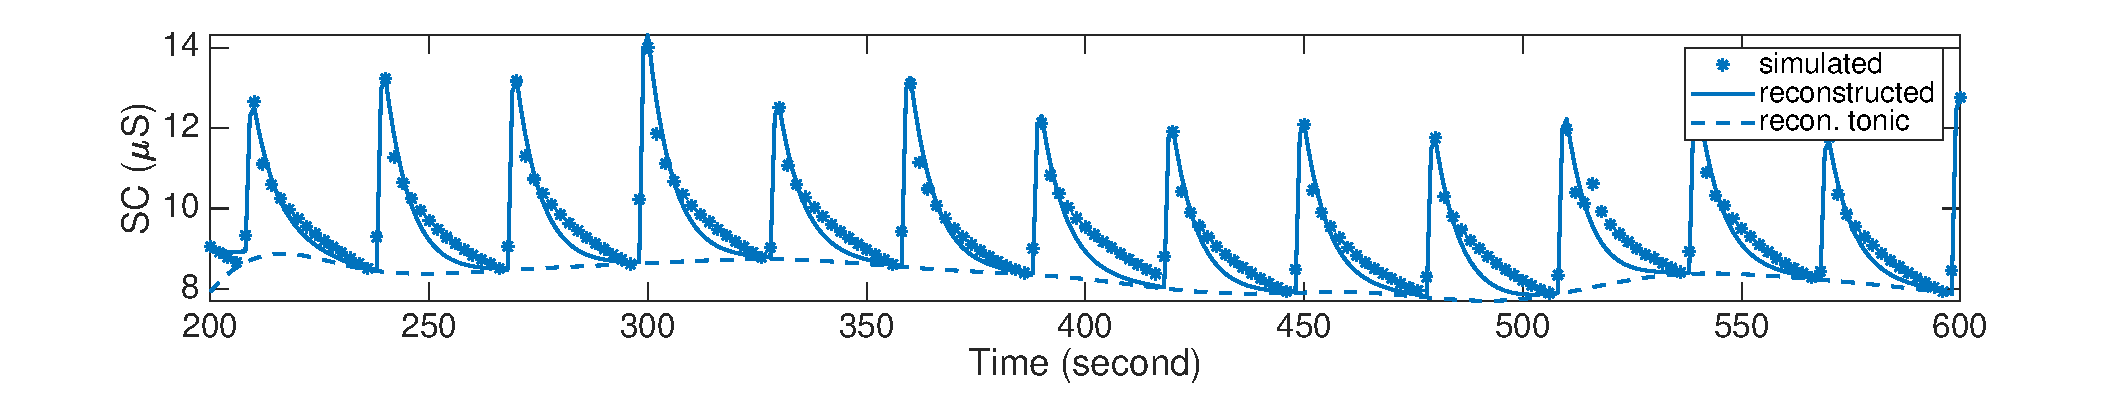
\includegraphics[width=0.9\textwidth]{middle_phalanx}}
  \subfigure[Reconstructed signal for the medial plantar surface data.]{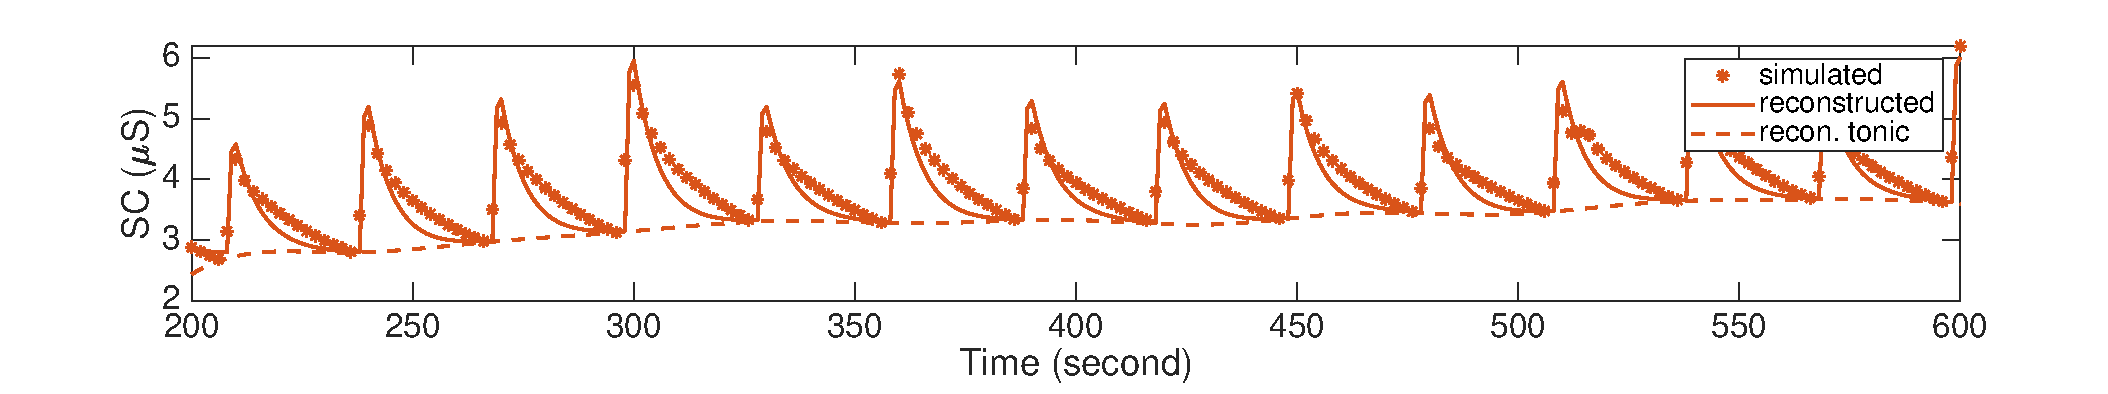
\includegraphics[width=0.9\textwidth]{medial_plantar}}
  \subfigure[The solved neural stimuli]{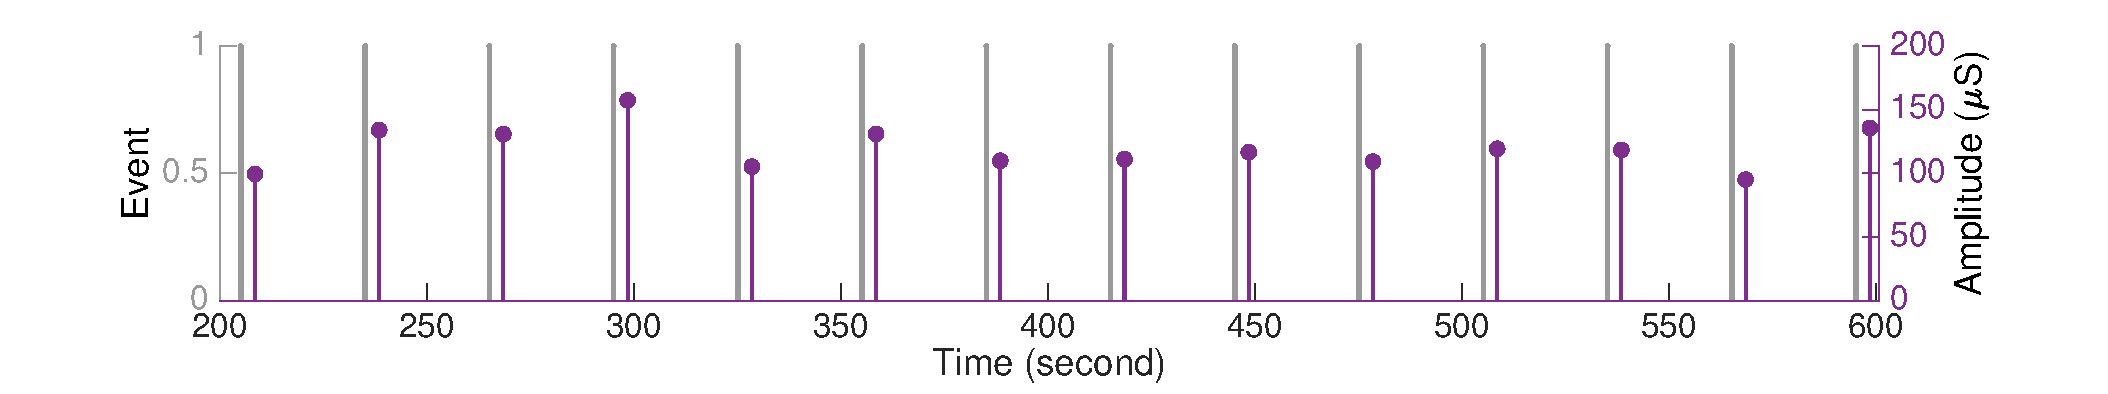
\includegraphics[width=0.9\textwidth]{stimuli} \label{fig:stimuli}}
  \DeclareGraphicsExtensions.
  \caption{The solution for the data collected from the $11^{\mathrm{th}}$ participant.} \label{fig:results}
\end{figure*}

The dataset used in this work is called \texttt{PsPM-SCRV10}\cite{bach2014pspm}, where ``\texttt{PsPM}'' is the abbreviation of the organization ``Psycho-Physiological Modelling'', and ``\texttt{SCRV\_10}'' is the symbolic name of the dataset. This dataset is collected from an experiment. 26 volunteers (12 males and 14 females) are invited for participating the test. The researchers produce a series white noise bursts as auditory stimulations. In response, the participants are required to press a food pedal every time they hear the burst. The data is recorded by Cambridge Electronic Design (CED) spike software.

According to the type of the data, the dataset could be divided into two parts. The first part is called ``cogent''. It contains the record about the participants' reactions including which pedal they press and how long the pedal is pressed. This part is not related to our work. The second part is called ``spikes''. It is a collection of skin conductance response (SCR) measurements. We only use the following parts of the data:

\begin{enumerate}
  \item Marker denoting timings of the auditory stimulations;
  \item Skin conductance on the thenar/hypothenar of the non-dominant hand;
  \item Skin conductance on the volar middle phalanx of the dominant 2nd/3rd finger;
  \item Skin conductance on the medial plantar surface of the non-dominant foot;
\end{enumerate}

Since each volunteer could provides 3 SC data, we construct our model as a 3-channel one. The marker denoting the auditory stimulations are used as the ground truth for estimating our results.

To simplify the calculation, we down sample the data by setting $T_y=1\rm{s}$. The bin sizes of the stimuli $T_u$ and the tonic coefficient $T_s$ are configured as 4s and 5s respectively. We take the results of the participant 11 as an example, where we extract the data from 200s to 600s. The results are shown in \cref{fig:results}. In \cref{fig:stimuli}, we draw the ground truth of the stimulation as gray bars and the solved neural stimuli as purple pins. The results show that the stimuli are always a little bit later than the stimulation. This phenomenon is reasonable, because there may be a latency caused by the physiological reactions.

\section{Discussion}

It is tricky to incorporate the tonic component extraction into the multi-channel deconvolution problem. Our basic idea is, when solving one component, view the other component as a constant variable and subtract it from the raw data. For example, when we solve the tonic component, intuitively the data with phasic component removed should be represented as
\begin{align}
  \mathbf{s}_n = \mathbf{y}_n - \mathcal{F}_{\boldsymbol{\theta}_n} \mathbf{z}_{0} - \mathcal{D}_{\boldsymbol{\theta}_n} \mathbf{u}.
\end{align}

In practice, we do not apply this method. Instead, we use \eqref{fml:the:second-tonic-obj} to calculate the objective data of the tonic component. This technique makes use of the initial guess of the tonic component, and constrains the lower bound of the objective data. In practice, it is very important to add this constraint. Because the sum of the solved phasic component and the tonic component may be larger than the true data $\mathbf{y}_n$. Without this method, the phasic component would cause the upper bound of the tonic component get reduced in each iteration. As a result, the objective data of the phasic component would increase, because the tonic component decreases step-by-step, which causes the tonic component further decrease in the next step. In a severe case, the tonic component could get reduced to 0.

Although we introduce the \eqref{fml:the:second-tonic-obj} to tackle this problem, this is a technically solution, not well-supported by the theory. We may require to define the constraint of the tonic component more carefully, for example, the tonic component may require a lower bound,
\begin{align}
  \mathbf{s}_{(b)n} \preccurlyeq \mathbf{C}\mathbf{q}_n \preccurlyeq \mathbf{y}_n.
\end{align}

How to define the lower bound is important. In our work, we use the initial guess of the tonic component as the lower bound. There may be better methods for the definition. We may develop a better solution in the future works.

\section{Conclusion}

In this work, we try to combine the tonic component extraction and the multi-channel phasic component deconvolution together. The problem is formulated as a joint problem for solving both components. To solve this problem, we use the concurrent coordinate descent method. For the phasic component, we formulate the model by a state-space representation, and use FOCUSS+ to solve the neural stimuli with sparsity regularization. In comparison, the tonic component is modeled by the decomposition of B-spline functions, we use the interior point method to solve the constrained quadratic problem. The regularization ratio for both components are estimated by the GCV method. The final results show that the phasic component and tonic component are separated, and the neural stimuli is well-regularized by the sparsity.

\bibliographystyle{ieeetr}
\bibliography{ref}

\end{document}